\documentclass[../../main.tex]{subfiles}
\begin{document}
\subsection*{Appendix II: Laplace Table}
\begin{longtable}{@{} CCC @{}}
    \toprule
    \multicolumn{2}{c}{$\begin{matrix} y = f (t), \quad t > 0 \\\\  y = f (t) = 0, t <0  \end{matrix}$}&Y = L(y) = F (p) \\
    \midrule
    \mathcal{L}1  & 1 & \begin{matrix} \dfrac{1}{p+a} \\\\  \text{Re }p>0  \end{matrix} \\\\
    \mathcal{L}2 &  e^{-at}  & \begin{matrix} \dfrac{1}{p} \\ \\ \text{Re }p>0 \end{matrix}  \\ \\
    \mathcal{L}3 &  \sin at &  \begin{matrix} \dfrac{a}{p^2+a^2} \\ \\ \text{Re }p>|\text{Im }a| \end{matrix} \\ \\
    \mathcal{L}4 &  \cos at &  \begin{matrix} \dfrac{p}{p^2+a^2} \\\\  \text{Re }p>|\text{Im }a|  \end{matrix} \\ \\
    \mathcal{L}5 &  t^k,\;k>-1 & \begin{matrix} \dfrac{k!}{p^{k+1}} \text{ or }\dfrac{\Gamma(k+1)}{p^{k+1}} \\\\  \quad \text{Re }p>0  \end{matrix}  \\ \\
    \mathcal{L}6 &  t^ke^{-at},\;k>-1 &  \begin{matrix} \dfrac{k!}{(p+a)^{k+1}} \text{ or }\dfrac{\Gamma(k+1)}{(p+a)^{k+1}}   \\\\  \text{Re }(p+a)>0 \end{matrix} \\ \\
    \mathcal{L}7 &  \dfrac{e^{-at} - e^{-bt}}{b-a} &  \begin{matrix} \dfrac{1}{(p+a)(p+b)}   \\\\  \text{Re }(p+a)>0 \\\text{Re }(p+b)>0  \end{matrix} \\ \\
    \mathcal{L}8 &  \dfrac{ae^{-at} - be^{-bt}}{b-a} & \begin{matrix} \dfrac{p}{(p+a)(p+b)}    \\\\  \text{Re }(p+a)>0 \\ \text{Re }(p+b)>0 \end{matrix}  \\ \\
    \mathcal{L}9 &  \sinh at & \begin{matrix} \dfrac{a}{p^2-a^2}  \\\\  \text{Re }p>|\text{Re }a|\end{matrix}\\ \\
    \mathcal{L}10 &  \cosh at &  \begin{matrix} \dfrac{p}{p^2-a^2} \\\\  \text{Re }p>|\text{Re }a|\end{matrix}\\ \\
    \mathcal{L}11 &   t\sin at  &  \begin{matrix} \dfrac{2ap}{(p^2+a^2)^2} \\\\ \text{Re }p>|\text{Im }a|\end{matrix} \\ \\
    \mathcal{L}12 &  t\cos at & \begin{matrix} \dfrac{p^2-a^2}{(p^2+a^2)^2} \\ \\ \text{Re }p>|\text{Im }a|\end{matrix} \\ \\
    \mathcal{L}13 &  e^{-at}\sin bt &  \begin{matrix} \dfrac{b}{(p+a)^2+b^2} \\\\ \text{Re }(p+a)>|\text{Im }b| \end{matrix}\\ \\
    \mathcal{L}14 &  e^{-at}\cos bt & \begin{matrix} \dfrac{p+a}{(p+a)^2+b^2} \\ \\ \text{Re }(p+a)>|\text{Im }b| \end{matrix}  \\ \\
    \mathcal{L}15 &  1 - \cos at & \begin{matrix}\dfrac{a^2}{p(p^2+a^2)} \\ \\ \text{Re }p>|\text{Im } a| \end{matrix} \\ \\
    \mathcal{L}16 &  at - \sin at &  \begin{matrix}\dfrac{a^3}{p^2(p^2+a^2)} \\ \\ \text{Re }p>|\text{Im } a|\end{matrix}\\ \\
    \mathcal{L}17 &  \sin at - at \cos at & \begin{matrix}\dfrac{2a^3}{(p^2+a^2)^2} \\ \\ \text{Re }p>|\text{Im } a| \end{matrix} \\ \\
    \mathcal{L}18 &  e^{-at}(1 - at)  & \begin{matrix} \dfrac{p}{(p+a)^2} \\ \\ \text{Re }(p+a)>0 \end{matrix} \\ \\
    \mathcal{L}19 &  \dfrac{\sin at}{t} & \begin{matrix}  \arctan \dfrac{a}{p} \\ \\ \text{Re }p>|\text{Im } a| \end{matrix}\\ \\
    \mathcal{L}20 &  \dfrac{1}{t}\sin at\cos bt & \begin{matrix} \dfrac{1}{2}\left(\arctan \dfrac{a+b}{p} +\arctan \dfrac{a-b}{p}\right) \\ \\ \text{Re }p>0\end{matrix} \\ \\
    \mathcal{L}21 &  \dfrac{e^{at}-e^{-bt}}{t} &  \begin{matrix}\ln\dfrac{p+b}{p+a} \\ \\ \text{Re }(p+a)>0 \\ \text{Re }(p+b)>0 \end{matrix}\\ \\
    \mathcal{L}22 &  \begin{matrix}1-\erf\left(\dfrac{a}{2\sqrt{t}}\right) \\ \\a>0 \end{matrix}&  \begin{matrix} \dfrac{1}{p}e^{-a\sqrt{p}} \\ \\ \text{Re }p>0 \end{matrix}\\ \\
    \mathcal{L}23 &  J_0(at) &  \begin{matrix}(p^2+a^2)^{-1/2} \\ \\ \text{Re }p>|\text{Im }a| \\ \text{Re }p\geq 0\\ \text{for real }a\neq0 \end{matrix}\\ \\
    \mathcal{L}24 &  \begin{matrix}\text{unit step,}\\ \text{Heaviside function} \\ u(t-a)=\begin{cases} 1,\\t>a>0&\\0,\; t<a& \end{cases}\\&\\\end{matrix} & \begin{matrix} \dfrac{1}{p}e^{-pa} \\ \\ \text{Re }p>0 \end{matrix}\\ \\
    \mathcal{L}25 & \begin{matrix}f(t)=u(t-a)-u(t-b)\\ 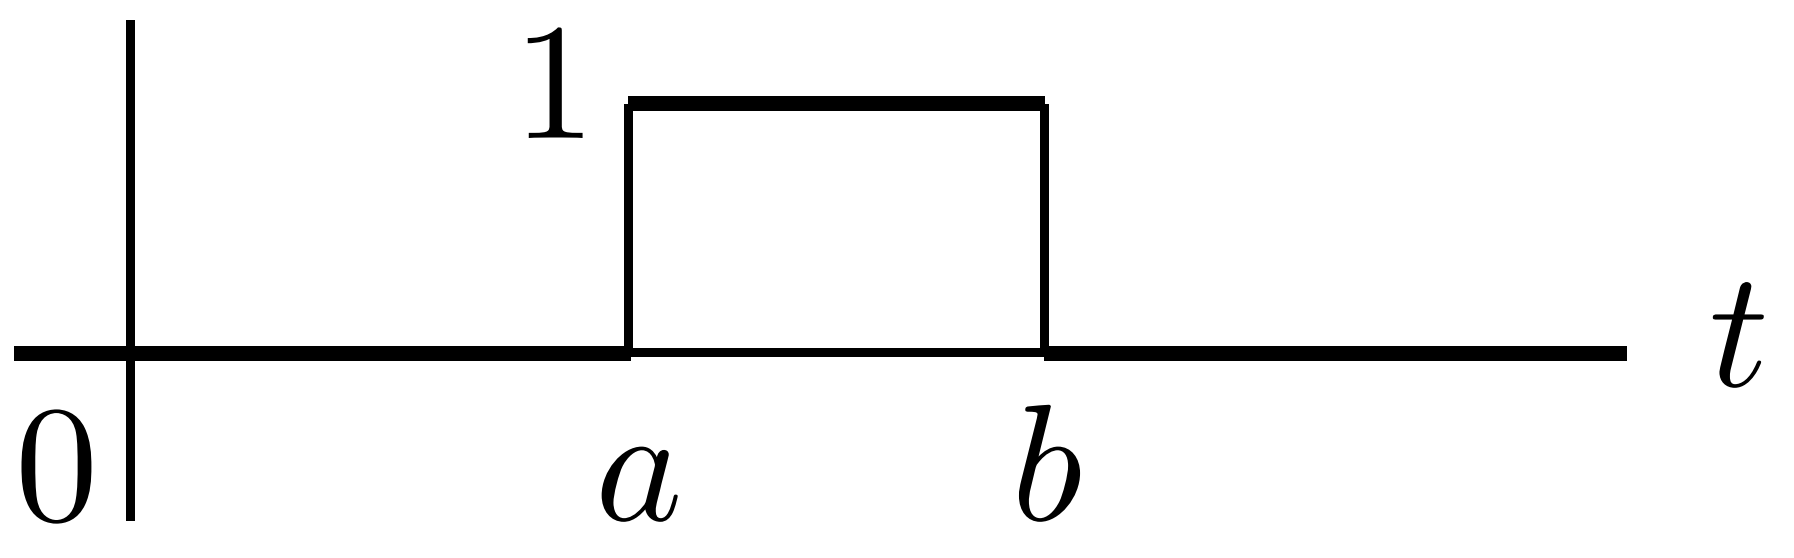
\includegraphics[width=0.3\textwidth]{../Rss/ODE/L25} \end{matrix}
   &  \begin{matrix}\dfrac{e^{-ap}-e^-bp}{p}  \\ \\\text{All }p\end{matrix}\\ \\
    \mathcal{L}26 &\begin{matrix}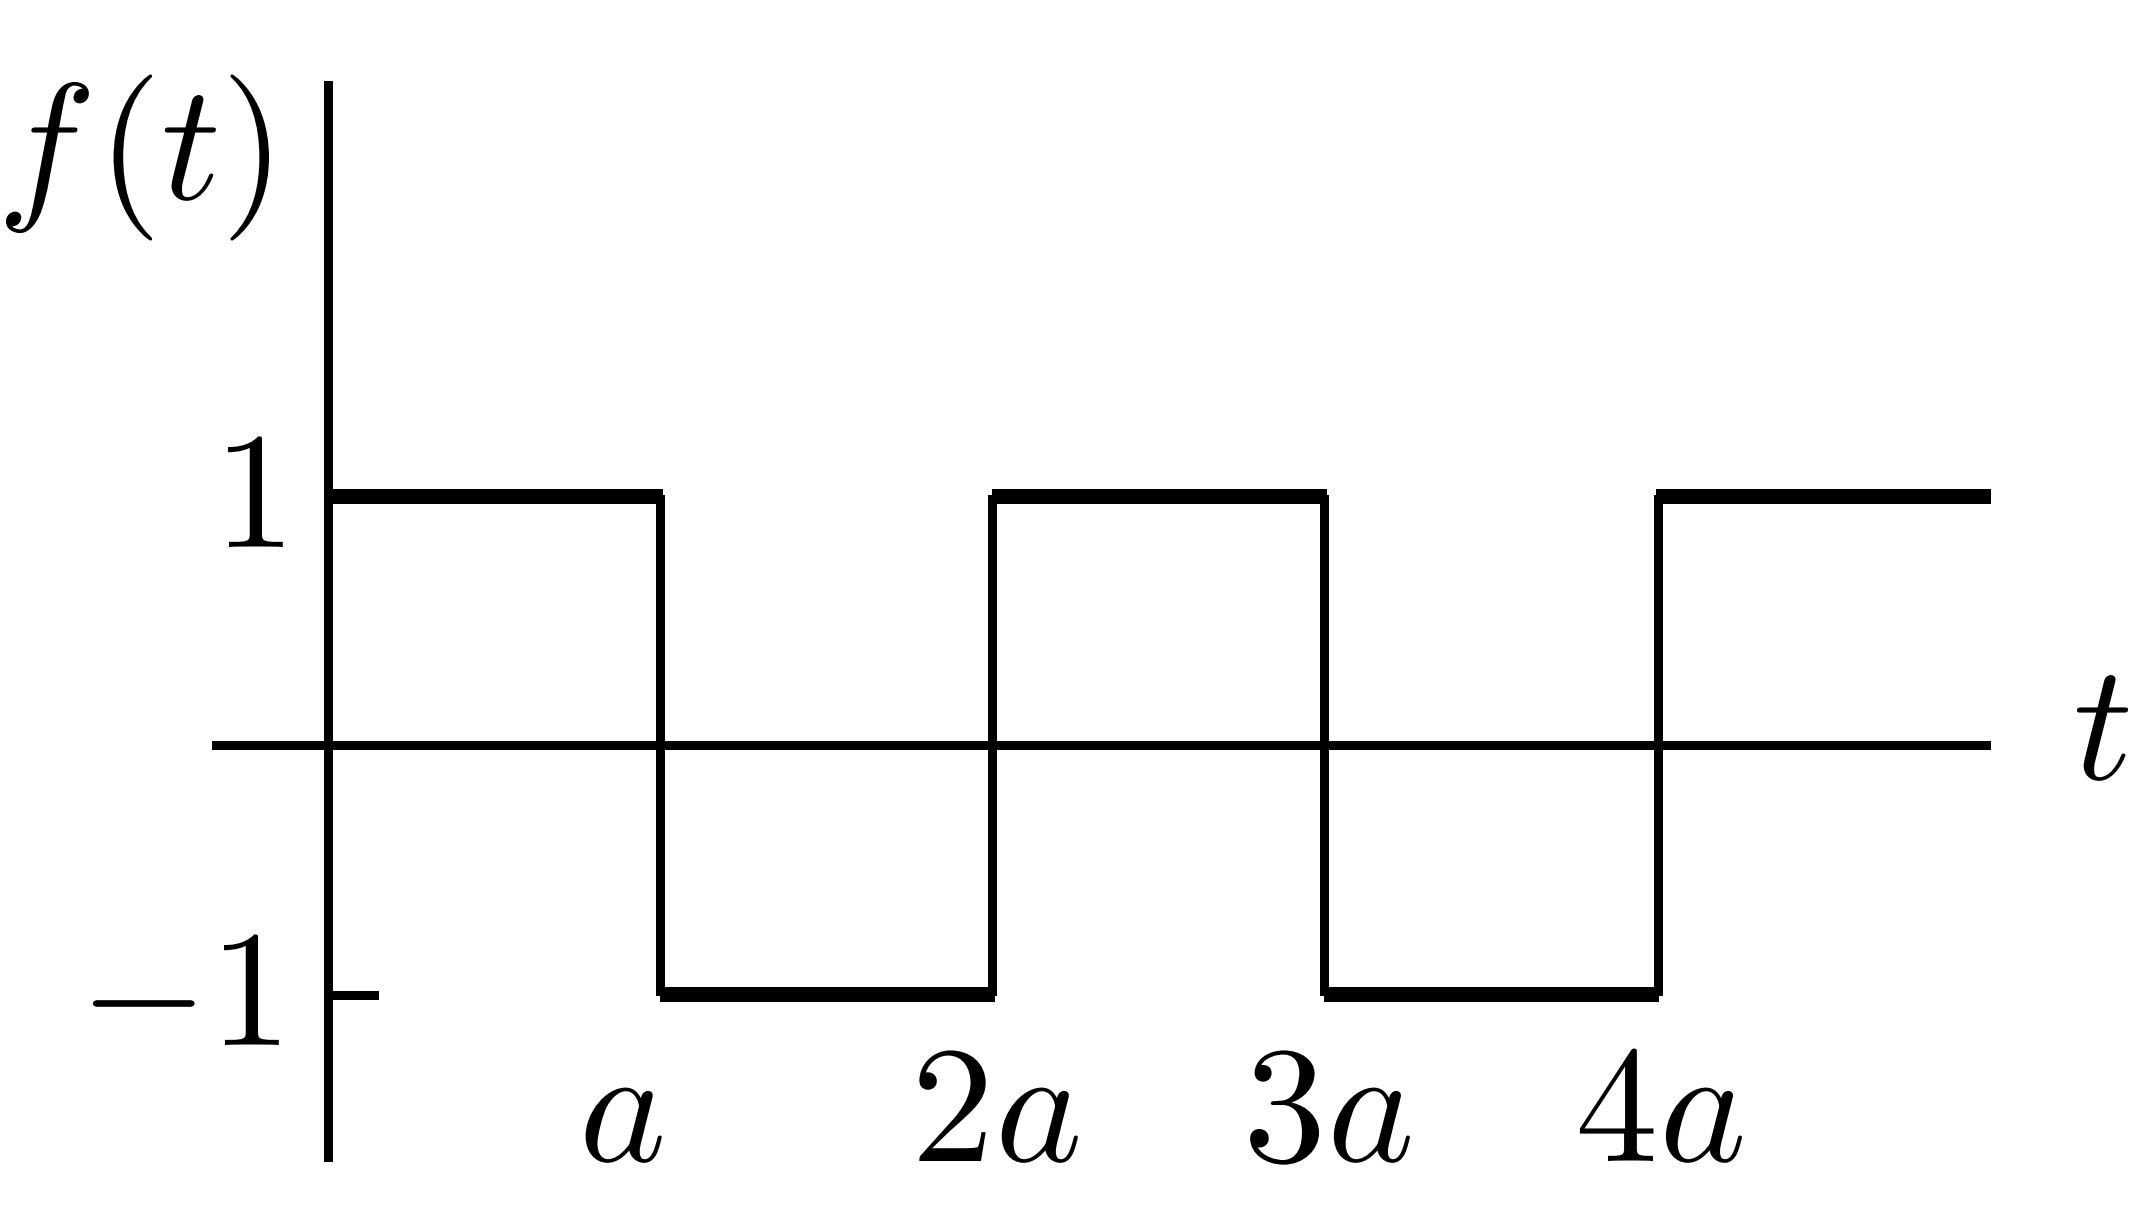
\includegraphics[width=0.3\textwidth]{../Rss/ODE/L26}\end{matrix}& \begin{matrix} \dfrac{1}{p}\tanh \frac{ap}{2} \\\\ \text{All }p \end{matrix}\\ \\
    \mathcal{L}27 & \displaystyle{  \delta(t-a),\;a\geq0} & \displaystyle{ e^{-pa}}\\ \\
    \mathcal{L}28 &\begin{matrix}f(t)=\begin{cases}g(t-a), &t>a>0\\0,&t<a \end{cases}\\ \\
        f(t) =g(t-a)u(t-a)\end{matrix} &\begin{matrix} e^{-pa}G(p)\\ \\ G(p) \text{ means } \mathcal{L}(g) \\\\\text{Therefore }e^{-pa}\mathcal{L}\left[g(t-a)\right] \end{matrix}\\ \\
    \mathcal{L}29 & \displaystyle{ e^{-at}g(t) } & \displaystyle{  G(p+a)}\\ \\
    \mathcal{L}30 &\displaystyle{  g(at),a>0} & \displaystyle{  \dfrac{1}{a}G\left(\frac{p}{a}\right)}\\ \\
    \mathcal{L}31 & \displaystyle{  \frac{g(t)}{t}}\text{ if integrable} & \displaystyle{  \int_{p}^{\infty}G(u)\;du}\\ \\
    \mathcal{L}32 & \displaystyle{ {t^n g(t) }} & \displaystyle{ {(-1)^n {\left(\frac{d}{dp}\right)}^n (G(p))}}\\ \\
    \mathcal{L}33 &\displaystyle{ \int_{0}^{t }g(\tau)\;d\tau } & {  \dfrac{1}{p}G(p)}\\ \\
    \mathcal{L}34 & \begin{matrix}\text{Convolution of $g$ and $h$,}\\\text{often written as}\\\displaystyle{g*h} \\ \displaystyle{=\int_{0}^{t}g(t-\tau)h(\tau)\;d\tau}\\\displaystyle{= \int_{0}^{t}g(\tau)h(t-\tau)\;d\tau } \end{matrix}& {  G(p)H(p)}\\ \\
    \mathcal{L}35 &\multicolumn{2}{c}{$\begin{matrix}\text{Transforms of derivatives of }y \\\\
            \begin{matrix}
                \mathcal{L}(y') &= &pY - y\\
                \mathcal{L}(y'') &=& p^2Y -p y_0-y_0'\\
                \mathcal{L}(y''') &=& p^3Y -p^2y_0-py_0'-y_0\\
                \mathcal{L}(y^n) &= &p^nY -p^{n-1} y_0-p^{n-2}y_0'-\dots-y_0^{n-1}  
            \end{matrix}
        \end{matrix}$}\\
    \bottomrule
\end{longtable}
\end{document}
